\documentclass{article}

% Use final NeurIPS (two-column)
\usepackage[final]{neurips_2022}

% Basics
\usepackage[utf8]{inputenc}
\usepackage[T1]{fontenc}
\usepackage{microtype}
\usepackage{hyperref}
\usepackage{url}
\usepackage{amsmath,amssymb}
\usepackage{booktabs}
\usepackage{xcolor}

% Algorithm package
\usepackage[ruled,vlined,linesnumbered]{algorithm2e}

% Floats/graphics
\usepackage{caption}
\captionsetup{font=small}
\setlength{\textfloatsep}{6pt plus 2pt minus 2pt}
\setlength{\abovecaptionskip}{3pt}
\setlength{\belowcaptionskip}{0pt}

\usepackage{tikz}
\usetikzlibrary{positioning,arrows.meta}

% Define argmin operator
\DeclareMathOperator*{\argmin}{arg\,min}
\DeclareMathOperator*{\argmax}{arg\,max}

\title{Project Milestone --- Literature Review:\\ A Dual--SPMA Framework for Convex MDPs}

\author{
Shervin Khamooshian \quad Ahmed Magd \quad Pegah Aryadoost \quad Danielle Nguyen\\
Simon Fraser University \qquad \texttt{\{ska309, ams80, paa40, tdn8\}@sfu.ca}
}

\begin{document}
\maketitle

% ============================================================================
% SECTION 1: PROJECT TOPIC
% ============================================================================
\section{Project Topic}

\textbf{Goal.} We study a unified way to solve \emph{Constrained Markov Decision Processes (CMDPs)} by combining a Fenchel-dual saddle formulation with a geometry-aware policy optimizer, \emph{Softmax Policy Mirror Ascent (SPMA)}. CMDPs minimize a convex function of discounted occupancies and are equivalent to the saddle problem:
\[
\min_{\pi}\max_{y}\ \langle y,d_{\pi}\rangle-f^*(y).
\]
Fixing $y$ turns the policy step into standard RL with shaped reward $r_y(s,a)=-y(s,a)$ (or $-\,\phi(s,a)^\top y$ under features). We alternate a mirror-ascent step on $y$ with an SPMA policy step and return discounted occupancy (or feature-expectation) estimates for the next dual update.

\textbf{Implementation.} Building on Zahavy's formulation, we alternate a dual step 
\[
y_{k+1}\!\leftarrow\!\text{MA}\!\left(y_k,\,\hat{d}_{\pi_k}-\nabla f^*(y_k)\right)
\] 
with a policy step that runs SPMA on the shaped reward $r_{y_k}=-y_k$, returning discounted occupancies $\hat{d}_{\pi_k}$ (or feature expectations) for the next dual update (Fig.~\ref{fig:dualspma}). We will benchmark this Dual--SPMA against NPG--PD, focusing on convergence speed, constraint satisfaction, and sample efficiency.

\begin{figure}[htbp]
\centering
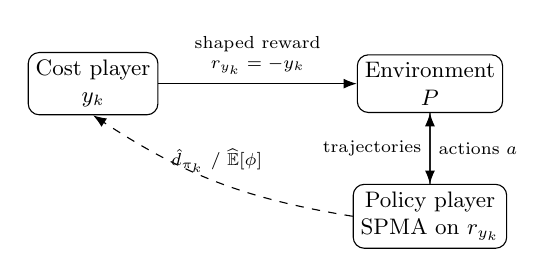
\begin{tikzpicture}[node distance=1cm, >=Latex, scale=0.9, transform shape]
\node[draw, rounded corners, align=center, inner sep=3pt, font=\small] (cost) {Cost player\\$y_k$};
\node[draw, rounded corners, align=center, inner sep=3pt, font=\small, right=2.8cm of cost] (env) {Environment\\$P$};
\node[draw, rounded corners, align=center, inner sep=3pt, font=\small, below=1cm of env] (policy) {Policy player\\SPMA on $r_{y_k}$};
\draw[->] (cost) -- node[above, align=center, font=\scriptsize]{shaped reward\\$r_{y_k}=-y_k$} (env);
\draw[->] (policy) -- node[right, font=\scriptsize]{actions $a$} (env);
\draw[->] (env) -- node[left, font=\scriptsize]{trajectories} (policy);
\draw[->, dashed, bend left=12] (policy.west) to node[above, font=\scriptsize]{$\hat d_{\pi_k}$ / $\widehat{\mathbb E}[\phi]$} (cost.south);
\end{tikzpicture}
\caption{\textbf{Dual--SPMA algorithm loop.} Dual ascent chooses $y_k$, which induces a shaped reward for the SPMA policy step; discounted occupancies feed the next dual update.}
\label{fig:dualspma}
\end{figure}

% ============================================================================
% SECTION 2: LITERATURE REVIEW - PAPER SUMMARIES
% ============================================================================
\section{Literature Review: Paper Summaries}

We review three foundational papers that inform our Dual--SPMA framework: (1) the Fenchel duality approach for convex MDPs, (2) the SPMA policy optimizer with fast convergence, and (3) primal-dual methods for constrained MDPs.

% ──────────────────────────────────────────────────────────────────────────
\subsection{Paper 1: \emph{Reward is Enough for Convex MDPs} (NeurIPS 2021)}

\textbf{Core idea.} Many RL goals can be posed as $\min_{d\in\mathcal{K}} f(d)$ for convex $f$ over the occupancy polytope $\mathcal{K}$. Using Fenchel conjugacy,
\[
\min_{d\in \mathcal{K}} f(d)=\min_{d\in \mathcal{K}}\max_{\lambda\in\Lambda}\ \lambda\!\cdot\! d - f^*(\lambda),
\]
so for fixed $\lambda$ the policy subproblem is vanilla RL with shaped reward $r_\lambda=-\lambda$.

Figure~\ref{fig:convex_mdp_game} illustrates this as a two-player game where the agent sees non-stationary rewards from the cost player. A meta-algorithm (Algorithm~\ref{alg:convex_mdp_meta}) alternates a \emph{cost player} (FTL/OMD in $\lambda$, a convex ascent step) with a \emph{policy player} (best response or low-regret RL), yielding $O(1/\sqrt{K})$ optimization error for averaged iterates under standard OCO assumptions. The paper shows best-response is ideal but often intractable in deep RL, so low-regret learners (e.g., UCRL2, MDPO) suffice; the guarantees hold for averaged occupancies $\bar{d}_\pi^K$ rather than single iterates. It unifies apprenticeship learning, CMDPs and pure exploration (Table~\ref{tab:convex_mdp_examples}). \citep{zahavy2021reward}

\begin{figure}[htbp]
\centering
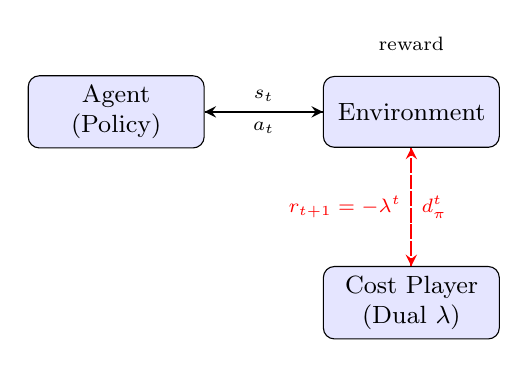
\begin{tikzpicture}[
    node distance=1.5cm,
    block/.style={rectangle, draw, fill=blue!10, text width=2cm, text centered, 
                  minimum height=0.9cm, rounded corners, font=\small},
    arrow/.style={->, >=stealth, thick}
]
\node[block] (agent) {Agent\\(Policy)};
\node[block, right=of agent] (env) {Environment};
\node[block, below=1.5cm of env] (cost) {Cost Player\\(Dual $\lambda$)};
\draw[arrow] (env) -- node[above, font=\scriptsize] {$s_t$} (agent);
\draw[arrow] (agent) -- node[below, font=\scriptsize] {$a_t$} (env);
\draw[arrow, dashed, red, thick] (cost) -- node[left, font=\scriptsize] {$r_{t+1} = -\lambda^t$} (env);
\draw[arrow, dashed, red, thick] (env) -- node[right, font=\scriptsize] {$d_\pi^t$} (cost);
\node[above=0.2cm of env, font=\scriptsize] {reward};
\end{tikzpicture}
\caption{Convex MDP as a two-player game (adapted from \citet{zahavy2021reward}, Fig.~1). The cost player provides shaped rewards $r_t = -\lambda^t$ to the agent, observing occupancy measures $d_\pi^t$.}
\label{fig:convex_mdp_game}
\end{figure}

\begin{algorithm}[t]
\caption{Meta-algorithm for Convex MDPs \citep{zahavy2021reward}}
\label{alg:convex_mdp_meta}
\small
\KwIn{Convex-concave payoff $\mathcal{L}: \mathcal{K} \times \Lambda \to \mathbb{R}$, algorithms $\text{Alg}_\lambda$, $\text{Alg}_\pi$, $K \in \mathbb{N}$}
\For{$k = 1, \ldots, K$}{
    $\lambda^k \leftarrow \text{Alg}_\lambda(d_\pi^1, \ldots, d_\pi^{k-1}; \mathcal{L})$ \tcp*{Cost player}
    $d_\pi^k \leftarrow \text{Alg}_\pi(-\lambda^k)$ \tcp*{Policy: RL with $r = -\lambda^k$}
}
\KwOut{$\bar{d}_\pi^K = \frac{1}{K}\sum_{k=1}^K d_\pi^k$, $\bar{\lambda}^K = \frac{1}{K}\sum_{k=1}^K \lambda^k$}
\end{algorithm}

\begin{table}[htbp]
\centering
\caption{Instantiations of the convex MDP framework (adapted from \citet{zahavy2021reward}, Table~1).}
\label{tab:convex_mdp_examples}
\small
\setlength{\tabcolsep}{2.5pt}
\begin{tabular}{@{}p{3.2cm}p{3.8cm}p{2.5cm}p{3cm}@{}}
\toprule
\textbf{Application} & \textbf{Objective $f(d_\pi)$} & \textbf{Cost Player} & \textbf{Policy Player} \\
\midrule
Standard RL & $-\lambda \cdot d_\pi$ & FTL & RL \\
Apprenticeship Learning & $\|d_\pi - d_E\|_2^2$ & FTL & Best Response \\
Pure Exploration & $d_\pi \cdot \log(d_\pi)$ & FTL & Best Response \\
Constrained MDPs & $\lambda_1 \cdot d_\pi$ s.t. $\lambda_2 \cdot d_\pi \leq c$ & OMD & RL \\
GAIL / State Matching & $\text{KL}(d_\pi \| d_E)$ & FTL & RL \\
\bottomrule
\end{tabular}
\end{table}

\textbf{Relevance to our project.} This work justifies the saddle formulation and the shaped-reward reduction we implement. It informs our outer-loop design (dual mirror ascent + policy best response).

% ──────────────────────────────────────────────────────────────────────────
\subsection{Paper 2: \emph{Fast Convergence of Softmax Policy Mirror Ascent} (OPT 2024 / arXiv 2025)}

\textbf{Core idea.} \emph{SPMA} performs mirror ascent in \emph{logit} space using the log-sum-exp mirror map, in contrast to NPG which uses exponential reweighting in probability space (Sec.~3.2). In tabular MDPs the per-state update (Eq.~3)
\[
\pi_{t+1}(a|s)=\pi_t(a|s)\bigl(1+\eta\,A^{\pi_t}(s,a)\bigr)
\]
avoids explicit normalization and achieves \emph{linear convergence} for sufficiently small constant step-size: bandit linear convergence (Thm.~1) and tabular MDP linear convergence to the optimal value (Thm.~2), improving over softmax PG (Sec.~3.3). 

For large problems, SPMA projects onto function classes via convex \emph{softmax classification} subproblems (Eq.~4--5, Algorithm~1):
\[
\theta_{t+1} = \argmin_\theta \sum_s d_{\pi_t}(s)\,
\mathrm{KL}\bigl(\pi_{t+1/2}(\cdot|s)\,\big|\,\pi_\theta(\cdot|s)\bigr).
\]
It proves linear convergence to a neighbourhood under FA (Sec.~4); the theory assumes exact or low-noise gradients, and performance depends on advantage-estimation quality (Sec.~4.2). Empirically it competes with PPO/TRPO/MDPO (Sec.~4.1). \citep{asad2024fast}

\textbf{Relevance to our project.} We need a strong policy ``best response'' in Zahavy's saddle; SPMA provides the geometry and fast rates in tabular settings, plus a practical FA implementation (convex surrogates that fit deep RL) matching our shaped-reward reduction.

% ──────────────────────────────────────────────────────────────────────────
\subsection{Paper 3: \emph{Natural Policy Gradient Primal--Dual for CMDPs} (NeurIPS 2020)}

\textbf{Core idea.} A policy-based primal--dual method for the Lagrangian CMDP formulation $V_r^\pi(\rho)+\lambda(V_g^\pi(\rho)-b)$: \emph{natural policy gradient} (NPG) ascent for the policy and projected subgradient updates for the multiplier (Eq.~7--8, Sec.~3--4), showing a multiplicative update for softmax policies and projection for $\lambda$. 

Despite nonconcavity/nonconvexity under softmax parameterization, it proves \emph{dimension-free} $O(1/\sqrt{T})$ bounds on averaged optimality gap and constraint violation (Thm.~1, Eq.~9a--9b) under Slater's condition; with FA, rates hold up to an approximation neighbourhood (Sec.~5, Thm.~3); sample-based variants have finite-sample guarantees (Thm.~4). \citep{ding2020npgpd}

\textbf{Relevance to our project.} NPG--PD is our principled CMDP baseline for both guarantees and practice: we compare Dual--SPMA (Fenchel saddle + SPMA policy player) against NPG--PD (Lagrangian saddle + NPG) in terms of geometry (logit-space vs.\ probability-space), convergence rates, constraint violation, and sample-efficiency.

% ============================================================================
% SECTION 3: HOW THE PAPERS RELATE TO EACH OTHER
% ============================================================================
\section{How the Papers Relate to Each Other}

The three papers provide complementary perspectives on our Dual--SPMA framework (Fig.~\ref{fig:framework_overview}):

\textbf{Formulation.} Zahavy et~al.\ provide the \emph{outer-loop template}: the Fenchel-dual saddle formulation that reduces constrained/structured RL to alternating between a cost player (dual ascent) and a policy player (shaped-reward RL). This formulation is key because fixing the dual variable $y$ yields standard RL with shaped reward $r_y = -y$.

\textbf{Policy player.} SPMA (Asad et~al.) supplies the \emph{fast policy player} for the RL step in Zahavy's framework. It performs mirror ascent in logit space, achieving linear convergence rates in tabular settings and practical function approximation via convex softmax classification. This makes SPMA an ideal candidate for the policy subproblem.

\textbf{Baseline and dual updates.} NPG--PD (Ding et~al.) offers a \emph{policy-based CMDP baseline} with dimension-free sublinear guarantees. While we use SPMA (not NPG) as our policy player, Ding et~al.\ inform how we handle constraint multipliers via projected subgradient updates and serve as our principled comparison baseline.

Table~\ref{tab:comparison} summarizes how these three approaches differ in their formulation, policy optimization method, and convergence guarantees.

\begin{figure}[t]
\centering
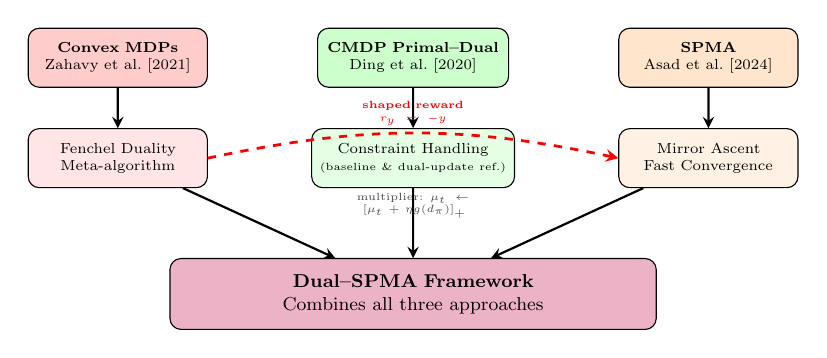
\begin{tikzpicture}[
    block/.style={rectangle, draw, text width=2.8cm, text centered, rounded corners, minimum height=1cm, font=\scriptsize},
    arrow/.style={->, >=stealth, thick},
    scale=0.75, transform shape
]

% Top row: Three source papers
\node[block, fill=red!20] (paper1) at (0,4.5) {
    \textbf{Convex MDPs}\\
    Zahavy et al.\ [2021]
};
\node[block, fill=green!20, text width=3cm] (paper2) at (5,4.5) {
    \textbf{CMDP Primal--Dual}\\
    Ding et al.\ [2020]
};
\node[block, fill=orange!20] (paper3) at (10,4.5) {
    \textbf{SPMA}\\
    Asad et al.\ [2024]
};

% Middle row: Contributions
\node[block, fill=red!10] (contrib1) at (0,2.8) {
    Fenchel Duality\\
    Meta-algorithm
};
\node[block, fill=green!10, text width=3.2cm] (contrib2) at (5,2.8) {
    Constraint Handling\\
    {\tiny (baseline \& dual-update ref.)}
};
\node[block, fill=orange!10] (contrib3) at (10,2.8) {
    Mirror Ascent\\
    Fast Convergence
};

% Multiplier note
\node[font=\tiny, text width=3cm, align=center, text=black!70] at (5,2) {
    multiplier: $\mu_t \leftarrow [\mu_t + \eta g(d_\pi)]_+$
};

% Bottom: Our framework
\node[block, fill=purple!30, text width=8cm, minimum height=1.2cm, font=\small] (ours) at (5,0.5) {
    \textbf{Dual--SPMA Framework}\\
    Combines all three approaches
};

% Vertical arrows
\draw[arrow] (paper1) -- (contrib1);
\draw[arrow] (paper2) -- (contrib2);
\draw[arrow] (paper3) -- (contrib3);

% Key connection arrow
\draw[arrow, dashed, red, bend left=12, line width=1pt] (contrib1.east) to 
    node[above, font=\tiny, text width=2.5cm, align=center] {
        \textbf{shaped reward}\\
        $r_y = -y$
    } (contrib3.west);

% Arrows to framework
\draw[arrow] (contrib1) -- (ours);
\draw[arrow] (contrib2) -- (ours);
\draw[arrow] (contrib3) -- (ours);

\end{tikzpicture}
\caption{Overview of how the three papers inform our Dual--SPMA framework. The key insight is that Zahavy's shaped reward reduction ($r_y = -y$) enables us to use SPMA as the policy player, while Ding et al.\ inform our constraint handling and serve as a baseline.}
\label{fig:framework_overview}
\end{figure}

\begin{table}[t]
\centering
\caption{Comparison of the three approaches that inform our project.}
\label{tab:comparison}
\small
\setlength{\tabcolsep}{2pt}
\begin{tabular}{@{}p{2.5cm}p{3.5cm}p{2.5cm}p{3.5cm}@{}}
\toprule
\textbf{Work} & \textbf{Formulation} & \textbf{Policy Method} & \textbf{Guarantees} \\
\midrule
Zahavy et al.\ (2021) \citep{zahavy2021reward} & Fenchel dual: $\min_d \max_\lambda \lambda\! \cdot\! d - f^{*}(\lambda)$ & Best response / low-regret RL under $r=-\lambda$ & $O(1/\sqrt{K})$ via OCO \\[4pt]
Asad et al.\ (2024) \citep{asad2024fast} & RL inner step (fixed $y$) & SPMA: $\pi_{t+1}=\pi_t(1+\eta A)$ & Linear (tabular); neighbourhood (FA) \\[4pt]
Ding et al.\ (2020) \citep{ding2020npgpd} & Lagrangian: $\max_\pi \min_{\lambda\ge0} V_r^\pi+\lambda(V_g^\pi-b)$ & NPG + projected subgradient & Dimension-free $O(1/\sqrt{T})$ \\
\bottomrule
\end{tabular}
\end{table}

% ============================================================================
% SECTION 4: PROJECT IMPLEMENTATION AND EVALUATION
% ============================================================================
\section{Project Implementation and Evaluation}

\textbf{Method.} Our Dual--SPMA algorithm alternates:
\begin{enumerate}
\item \textbf{Dual update:} $y_{k+1}\!\leftarrow\!\text{MA}\!\left(y_k,\,\hat d_{\pi_k}-\nabla f^*(y_k)\right)$
\item \textbf{Policy step:} Run SPMA for $K_{\text{in}}$ epochs on shaped reward $r_{y_k}=-y_k$
\item \textbf{Return:} Discounted occupancies $\hat d_{\pi_k}$ (or $\widehat{\mathbb E}[\phi]$ under FA)
\end{enumerate}

\textbf{Evaluation metrics.} We will measure:
\begin{itemize}
\item[(i)] Saddle value $L(\pi,y)$ (when $f^*$ is known)
\item[(ii)] Constraint value and constraint violation
\item[(iii)] Policy return under shaped reward $r_y$
\item[(iv)] Convergence of $\|\hat d_{\pi}\|_1$ (tabular) or $\|\widehat{\mathbb E}[\phi]\|$ (FA)
\item[(v)] Wall-clock time and sample efficiency
\end{itemize}

\textbf{Baselines.} We will compare against NPG--PD (Ding et al., 2020) as our principled CMDP baseline, evaluating differences in convergence speed, constraint satisfaction, and sample efficiency.

\small
\bibliographystyle{abbrvnat}
\bibliography{refs}
\end{document}